\begin{frame}{Revisión de Residuales por Sensor}

    \begin{columns}[T]
        %========================================
        % COLUMNA IZQUIERDA: TABLA EXACTA
        %========================================
        \column{0.48\textwidth}
        \begin{block}{Tabla de Residuales (Datos Reales)}
            \centering
            \tiny % Usamos tiny para que quepan las 12 filas
            \begin{tabular}{@{}lcccc@{}}
                \toprule
                \textbf{Sen.} & \textbf{Obs.} & \textbf{Pred.} & \textbf{Resid.} & \textbf{|Res|} \\ \midrule
                S1  & 0.005219 & 0.005149 & 0.000070 & 0.000070 \\
                S2  & 0.009811 & 0.009999 & -0.000188 & 0.000188 \\
                S3  & 0.012014 & 0.012270 & -0.000256 & 0.000256 \\
                S4  & 0.024570 & 0.024087 & 0.000483 & 0.000483 \\
                S5  & 0.080580 & 0.079390 & 0.001190 & 0.001190 \\
                S6  & 0.071733 & 0.074057 & -0.002324 & 0.002324 \\
                S7  & 0.027704 & 0.026317 & 0.001387 & 0.001387 \\
                S8  & 0.003556 & 0.003598 & -0.000042 & 0.000042 \\
                S9  & 0.852201 & 0.852651 & -0.000450 & 0.000450 \\
                S10 & 0.380182 & 0.379389 & 0.000793 & 0.000793 \\
                S11 & 0.119785 & 0.115769 & 0.004016 & 0.004016 \\
                S12 & 0.037284 & 0.035687 & 0.001597 & 0.001597 \\ \bottomrule
            \end{tabular}
        \end{block}

        %========================================
        % COLUMNA DERECHA: IMAGEN Y CONCLUSIÓN
        %========================================
        \column{0.48\textwidth}
        \vspace{0.5cm}
        \begin{center}
            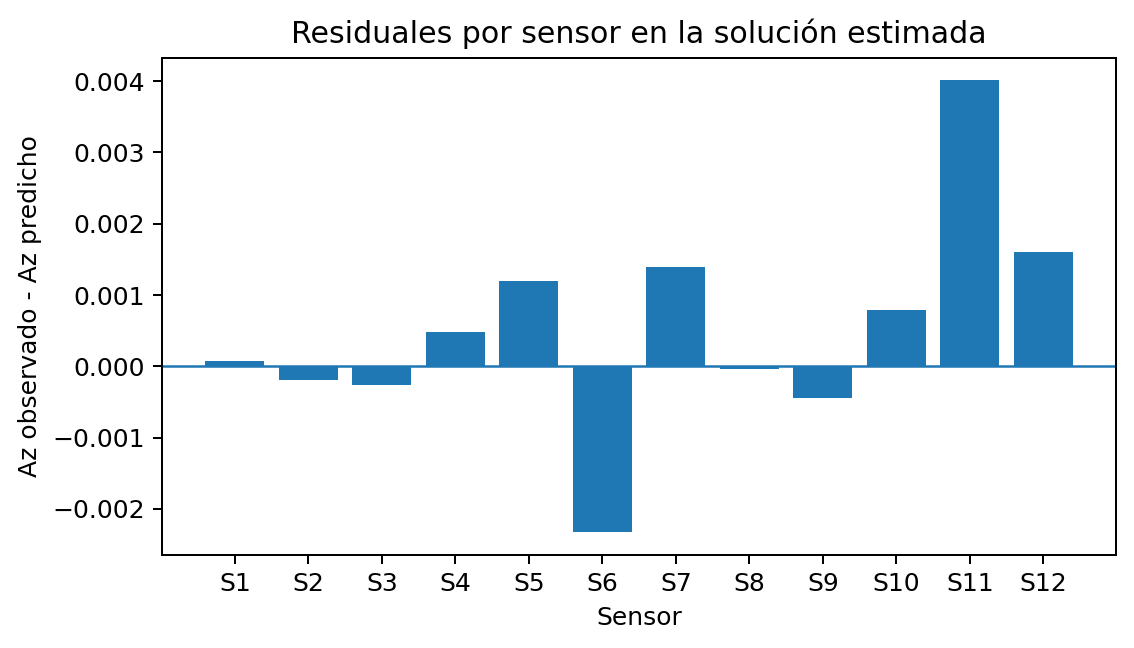
\includegraphics[width=\textwidth]{Imagenes/ResidualSensor.png}
            \\[0.2cm]
            \tiny \textcolor{gray}{Distribución de residuales por sensor.}
        \end{center}
        
        \vspace{-0.9cm}
        \begin{block}{Interpretación}
            \scriptsize
            La baja magnitud de los residuos (del orden de $10^{-3}$ a $10^{-4}$) confirma que el modelo propuesto tiene un ajuste preciso sobre la red de 12 sensores simulados.
        \end{block}
    \end{columns}

\end{frame}